\documentclass[a4paper]{article}
%% Language and font encodings
\usepackage[english]{babel}
\usepackage[utf8x]{inputenc}
\usepackage[T1]{fontenc}
\usepackage{float}
%% Sets page size and margins
\usepackage[a4paper,top=3cm,bottom=2cm,left=3cm,right=3cm,marginparwidth=1.75cm]{geometry}
\usepackage[caption=false]{subfig}
\setcounter{section}{-1}
%% Useful packages
\usepackage{fancyhdr}
\pagestyle{fancy}
\usepackage{amsmath}
\usepackage{amsthm}
\usepackage{enumitem}
\usepackage{eqnarray}
\usepackage{float}
\usepackage{esint}
\usepackage{wrapfig}
\usepackage{gensymb}
\usepackage{lipsum}
\usepackage{amssymb}
\usepackage{array}
\usepackage{tikz}
\usetikzlibrary{arrows,decorations.markings}
\usepackage[colorlinks=true, allcolors=blue]{hyperref}
\usepackage{graphicx}
\usepackage{amsmath}
\usepackage{amssymb}
\usepackage{graphicx}
\usepackage{mathtools}
\usepackage[colorlinks=true, allcolors=blue]{hyperref}
\DeclareMathOperator{\lcm}{lcm}
\DeclareMathOperator{\var}{Var}
\DeclareMathOperator{\sech}{sech}
\DeclareMathOperator{\cosech}{cosech}
\DeclareMathOperator{\cov}{Cov}
\DeclareMathOperator{\sgn}{sgn}
\DeclareMathOperator{\Span}{span}
\DeclareMathOperator{\nullity}{nullity}
\DeclareMathOperator{\rank}{rank}
\DeclareMathOperator{\Ker}{Ker}
\DeclareMathOperator{\R}{R}
\DeclareMathOperator{\Tr}{Tr}
\DeclareMathOperator{\sinc}{sinc}
\DeclareMathOperator{\diag}{diag}
\newtheorem{remarks}{Remarks}[section]
\newtheorem{eg}{Example}[section]
\newtheorem{Note}{Note}[section]
\definecolor{darkblue}{RGB}{	0, 0, 139}
\newtheoremstyle{new}% <name>
{2pt}% <Space above>
{2pt}% <Space below>
{\color{darkblue}}% Body font
{}% <Indent amount>
{\bfseries\color{black}}% Theorem head font
{:}% <Punctuation after theorem head>
{.5em}% <Space after theorem headi>
{}% <Theorem head spec (can be left empty, meaning `normal')>
\theoremstyle{new}
\newtheorem{law}{Law}[section]
\newtheorem{defi}{Definition}[section]
\newtheorem{thm}{Theorem}[section]
\newtheorem{prop}{Proposition}[section]
\newtheorem{lemma}{Lemma}[section]
\newtheorem{cor}{Corollary}[section]

\title{\textbf{EO (Electrodynamics and Optics) Part II Phy}}
\author{Tai Yingzhe, Tommy (ytt26)}
\date{}
\setlength{\parindent}{0cm}
\begin{document}
\maketitle
\tableofcontents
%5 lectures from DAMTP electrodynamics, self read antenna and scattering and optics

\newpage
\section{Review of IB Electromagnetism}
\begin{defi}[Dielectric]
A dielectric material has no mobile charges that can move freely in an applied field but they nevertheless have a significant effect on applied electric fields. 
\end{defi}
\begin{defi}[Polarization]
The dipole moment per unit volume is called polarization $\mathbf{P}$.
\end{defi}
\begin{defi}[Electric Displacement]
We define the electric displacement to be
$$\mathbf{D}=\varepsilon_0\mathbf{E}+\mathbf{P}$$
\end{defi}
\begin{defi}[Linear Dielectric]
For linear dielectrics, the induced polarization $\mathbf{P}$ is proportional to the externally applied electric field $\mathbf{E}$.
\end{defi}
\begin{defi}[Electric Susceptibility]
The electric susceptibility is the constant of proportionality for the linear dielectric relation.
$$\mathbf{P}=\varepsilon_0\chi_e\mathbf{E}$$
\end{defi}
\begin{defi}[Permittivity and Dielectric Constant]
We define the permittivity of the material to be $\varepsilon:=\varepsilon_0(1+\chi_e)$ and $\varepsilon_r:=1+\chi_e$.
\end{defi}
\begin{cor}
In a linear dielectric, the displacement is also proportional to the field.
\end{cor}
\begin{proof}
$\mathbf{D}=\varepsilon_0\mathbf{E}+\mathbf{P}=\varepsilon_0(1+\chi_e)\mathbf{E}=\varepsilon\mathbf{E}$.
\end{proof}
\begin{defi}[Magnetic Material]
All materials are in some sense magnetic since they contain microscopic, atomic-scale currents and magnets which are themselves sources of magnetic field. When magnetically polarized, the material develops a magnetization.
\end{defi}
\begin{defi}[Magnetization]
Magnetization is the magnetic dipole moment per unit volume.
$$\mathbf{M}:=\frac{\boldsymbol{m}}{V}$$
\end{defi}
\begin{defi}[Auxiliary Field]
We define the auxiliary field to be
$$\mathbf{H}=\frac{1}{\mu_0}\mathbf{B}-\mathbf{M}$$
\end{defi}
\begin{defi}[Linear Magnetic Material]
For linear magnetic media, $\mathbf{M}$ is directly proportional to $\mathbf{H}$.
\end{defi}
\begin{defi}[Magnetic Susceptibility]
The magnetic susceptibility is the constant of proportionality for the linear magnetic media relation.
$$\mathbf{M}=\chi_m\mathbf{H}$$
\end{defi}
\begin{defi}[Relative Permeability]
We define the relative permeability $\mu_r:=1+\chi_m$.
\end{defi}
\begin{cor}
In a linear magnetic medium, the magnetic field is also proportional to the auxiliary field.
\end{cor}
\begin{proof}
$\mathbf{B}=\mu_0(\mathbf{H}+\mathbf{M})=\mu_0(1+\chi_m)\mathbf{H}=\mu\mathbf{H}$.
\end{proof}
\begin{Note}[Maxwell's Macroscopic Equations]
The Maxwell's equations in matter are:
$$\varepsilon_0\boldsymbol{\nabla}\cdot\mathbf{E}=\rho_f+\rho_b=\rho_f-\boldsymbol{\nabla}\cdot\mathbf{P}\implies\int_{\mathcal{S}}\mathbf{D}\cdot d\mathbf{S}=\int_{\mathcal{V}}\rho_fdV,\quad\boldsymbol{\nabla}\cdot\mathbf{D}=\rho_f$$
$$\int_{\mathcal{S}}\mathbf{B}\cdot d\mathbf{S}=0,\quad \boldsymbol{\nabla}\cdot\mathbf{H}=0$$
$$\oint_{\mathcal{C}}\mathbf{E}\cdot d\mathbf{l}=-\frac{d}{dt}\int_{\mathcal{S}}\mathbf{B}\cdot d\mathbf{S},\quad \boldsymbol{\nabla}\times\mathbf{E}=-\frac{\partial\mathbf{B}}{\partial t}$$
$$\frac{1}{\mu_0}\boldsymbol{\nabla}\times\mathbf{B}=\mathbf{J_f}+\mathbf{J_m}+\mathbf{J_b}+\varepsilon_0\frac{\partial\mathbf{E}}{\partial t}\implies\oint_{\mathcal{C}}\mathbf{H}\cdot d\mathbf{l}=\int_{\mathcal{S}}\mathbf{J_f}\cdot d\mathbf{S}+\frac{d}{dt}\int_{\mathcal{S}}\mathbf{D}\cdot d\mathbf{S},\quad\boldsymbol{\nabla}\times\mathbf{H}=\mathbf{J_f}+\frac{\partial\mathbf{D}}{\partial t}$$
\end{Note}
\begin{prop}[Statement of Conservation of Charge]
Consider a domain $D$ with boundary $S=\partial D$, the rate of change of charge density $\rho$ is related to the current density $\mathbf{J}$:
$$\frac{\partial\rho}{\partial t}+\boldsymbol{\nabla}\cdot\mathbf{J}=0$$
\end{prop}
\begin{prop}[Poisson's Equation]
The scalar electric potential $\phi$ satisfies the Poisson's equation, which is a linear PDE.
$$\nabla^2\phi=-\rho/\varepsilon_0$$
\end{prop}
\begin{prop}
The energy density of an electromagnetic field in a material is
$$u=\frac{1}{2}\mathbf{E}\cdot\mathbf{D}+\frac{1}{2}\mathbf{B}\cdot\mathbf{H}$$
The Poynting vector for these waves are $\mathbf{N}=\mathbf{E}\times\mathbf{H}$.
\end{prop}
\begin{prop}
The fields $\mathbf{E}$ and $\mathbf{B}$ can be written in terms of the potentials $\phi$ and $\mathbf{A}$. 
$$\mathbf{B}=\boldsymbol{\nabla}\times\mathbf{A},\quad\mathbf{E}=-\boldsymbol{\nabla}\phi-\frac{\partial\mathbf{A}}{\partial t}$$
These potential have gauge freedom.
\end{prop}
\begin{Note}[Boundary Conditions]
$$B_{\text{top}}^{\perp}=B_{\text{bottom}}^{\perp},\quad E_{\text{top},\parallel}=E_{\text{bottom},\parallel}$$
$$D_{\text{top}}^{\perp}-D_{\text{bottom}}^{\perp}=\sigma_f,\quad H_{\text{top}}^{\parallel}-H_{\text{bottom}}^{\parallel}=\mathbf{K_f}\times\mathbf{\hat{n}}$$
\end{Note}
\begin{prop}[Electromagnetic Waves]
The solution to Maxwell's equations in the case where $\rho=0$ and $\mathbf{J}=0$ (free space) is the equation of electromagnetic waves.
\end{prop}
\begin{remarks}\leavevmode
\begin{enumerate}
    \item Complex wavevector $\mathbf{k}+i\boldsymbol{\kappa}$ would mean the EM waves are damped. If $\mathbf{k}$ is parallel to $\boldsymbol{\kappa}$, the EM wave is homogeneous. Otherwise, it is inhomogeneous.
    \item The EM waves satisfy
    $$\mathbf{k}\cdot\mathbf{D}=0,\quad\mathbf{k}\cdot\mathbf{B}=0$$
    $$\mathbf{k}\times\mathbf{E}=\omega\mathbf{B},\quad\mathbf{k}\times\mathbf{H}=-\omega\mathbf{D}$$
    i.e. $\{\mathbf{B},\mathbf{k},\mathbf{E}\}$ and $\{\mathbf{D},\mathbf{k},\mathbf{H}\}$ are separately mutually orthogonal sets, while $\mathbf{E}$ and $\mathbf{H}$ are not necessarily perpendicular to $\mathbf{k}$. (It is, if the material is isotropic.)
\end{enumerate}
\end{remarks}
\begin{prop}
Some of the incident light on the interface of a linear media will be reflected and some will be transmitted. For s-polarization (light polarized in a direction perpendicular to the plane of incidence), the reflection and transmission ratios will be:
$$
r_s=\frac{\cos(\theta_i)-\sqrt{(\frac{n_t}{n_i})^2-\sin^2(\theta_i)}}{\cos(\theta_i)+\sqrt{(\frac{n_t}{n_i})^2-\sin^2(\theta_i)}},\quad t_s=\frac{2\cos(\theta_i)}{\cos(\theta_i)+\sqrt{(\frac{n_t}{n_i})^2-\sin^2(\theta_i)}}$$
For p-polarization (light polarized in a direction parallel to the plane of incidence), the reflection and transmission ratios will be:
$$
r_p=\frac{-(\frac{n_t}{n_i})^2\cos(\theta_i)+\sqrt{(\frac{n_t}{n_i})^2-\sin^2(\theta_i)}}{(\frac{n_t}{n_i})^2\cos(\theta_i)+\sqrt{(\frac{n_t}{n_i})^2-\sin^2(\theta_i)}},\quad t_p=\frac{2\cos(\theta_i)}{(\frac{n_t}{n_i})^2\cos(\theta_i)+\sqrt{(\frac{n_t}{n_i})^2-\sin^2(\theta_i)}}$$
\end{prop}
\begin{defi}[Brewster's angle]
The Brewster's angle is the angle of incidence where the reflection coefficient for light polarized parallel to the plane of incidence being zero.
\end{defi}
\begin{prop}[Plasma oscillations]
At the plasma frequency $\omega=\omega_p$, $\varepsilon(\omega_p)=0$, the wave is longitudinal with $\mathbf{k}$ parallel to $\mathbf{E}$.
\end{prop}
\newpage
\section{Optics}
\subsection{Polarization}
\begin{defi}[Linearly Polarized Waves]
A solution with real $\mathbf{E_0}$, $\mathbf{B_0}$, $\mathbf{k}$ is said to be linearly polarized.
\end{defi}
\begin{defi}[Elliptically Polarized Waves]
If $\mathbf{E_0}$ and $\mathbf{B_0}$ are complex, then it is said to be elliptically polarized.
\end{defi}
\begin{defi}[Circularly Polarized Waves]
For an elliptically polarized wave, if $|\boldsymbol{\alpha}| = |\boldsymbol{\beta}|$ and $\boldsymbol{\alpha}\cdot\boldsymbol{\beta}=0$, where $\mathbf{E_0}=\boldsymbol{\alpha}+i\boldsymbol{\beta}$.
\end{defi}
\begin{eg}
Take
$$\mathbf{E_T}=E_0(\mathbf{\hat{x}}e^{i(kz-\omega t)}+\mathbf{\hat{y}}e^{i(kz-(\omega t-0.5\pi))})$$
then $E_y$ lags behind $E_x$ by $\delta=\pi/2$. This is defined as a left-handed circularly polarized wave (LCP). An observer towards whom the light is propagating sees $\mathbf{E_T}(z=0)$ rotates anti-clockwise.
\end{eg}
\begin{eg}
For $|a_1|\neq|a_2|$ and $\delta\neq\pm\pi/2$, $\mathbf{E}$ is elliptically polarized with the major/minor axes along directions in the $xy$ plane determined as follows. With $a_1=a$, $a_2=be^{i\delta}$ such that $a,b\in\mathbb{R}$:
$$E_x=a\cos\omega t,\quad E_y=b\cos(\omega t-\delta)$$
which gives
$$\frac{E_y}{b}=\cos\omega t\cos\delta+\sin\omega t\sin\delta=\frac{E_x}{a}\cos\delta+\bigg(1-\frac{E_x^2}{a^2}\bigg)^{1/2}\sin\delta\implies\frac{E_x^2}{a^2}+\frac{E_y^2}{b^2}-2\cos\delta\frac{E_x}{a}\frac{E_y}{b}=\sin^2\delta$$
where $\alpha=0.5\tan^{-1}\frac{2ab\cos\delta}{a^2-b^2}$ is the angle the ellipse's axes are inclined to with respect to $E_x$ and $E_y$ directions.
\end{eg}
\begin{defi}[Jones Notation]
The complex amplitudes $a_1$ and $a_2$ of the two $x$ and $y$ linearly polarized waves can be used as the basis for a useful matrix approach for handling the effect of various optical devices on the polarization state.
\end{defi}
\begin{eg}
By definition, $x$- and $y$-polarized light are represented by $(1,0)$ and $(0,1)$ respectively, while $\theta$-polarized light is represented by $(\cos\theta,\sin\theta)$. Right circularly polarized and left circularly polarized light respectively represented by $(1/\sqrt{2})(1,-i)$ and $(1/\sqrt{2})(1,i)$. A general elliptically polarized light will be represented by $(a,be^{i\delta})$. Linear combinations, with appropriate phases, of the various polarization states can be used to form other polarization states. For instance, adding both RCP and LCP waves gives $x$-polarized waves.
\end{eg}
\subsection{Anisotropic Media}
\subsubsection{Dichroism}
\begin{defi}[Dichroic materials]
Dichroic materials absorb light linearly polarized in one direction more than light polarized in the other.
\end{defi}
\begin{eg}
A polaroid film is a plastic containing conducting polymeric chains aligned by stretching. If the sheet is anisotropic, conducting along $\mathbf{\hat{y}}$ but not along $\mathbf{\hat{x}}$, then light with $\mathbf{E}$ parallel to $\mathbf{\hat{y}}$ is absorbed while those parallel to $\mathbf{\hat{x}}$ is not. The Jones matrix representation for this polaroid is
$$J_x=\begin{pmatrix}1&0\\0&0\\\end{pmatrix}$$
In general, a polaroid with transmitting axis oriented at $\theta$ to $\mathbf{\hat{x}}$ is represented by
$$J_\theta=\begin{pmatrix}\cos^2\theta&\sin\theta\cos\theta\\\sin\theta\cos\theta&\sin^2\theta\\\end{pmatrix}$$
\end{eg}
\begin{eg}[Malus's Law]
For initially $x$-polarized light of intensity $I_0$ which then passes through polarizer $J_\theta$, the output is
$$J_\theta L_x=\begin{pmatrix}\cos^2\theta&\sin\theta\cos\theta\\\sin\theta\cos\theta&\sin^2\theta\\\end{pmatrix}\begin{pmatrix}1\\0\\\end{pmatrix}\sqrt{I_0}$$
so the transmitted intensity is
$$I(\theta)=I_0(\cos^4\theta+\sin^2\theta\cos^2\theta)=I_0\cos^2\theta$$
\end{eg}
\subsubsection{Birefringence}
\begin{defi}[Birefringence]
Birefringence is the optical property of a material having a refractive index that depends on the polarization and propagation direction of light. These optically anisotropic materials are said to be birefringent. It can be found from
$$\Delta n=n_e-n_o$$
where $n_e$ and $n_o$ are refractive indices along the extraordinary and ordinary ray.
\end{defi}
\begin{defi}[Permittivity/dielectric tensor]
For a materials with an anisotropic crystal structure, $\mathbf{E}$ is not necessarily parallel to $\mathbf{D}$ and we thus require a rank two tensor for permittivity, i.e.
$$D_i=\varepsilon_0\sum_j\varepsilon_{ij}E_j$$
\end{defi}
\begin{prop}
If the system has no energy loss, the dielectric tensor must be Hermitian.
\end{prop}
\begin{proof}
We have the rate of change of energy density in a material to be
$$\frac{du}{dt}=\frac{1}{2}\frac{d}{dt}(\mathbf{E}\cdot\mathbf{D}+\mathbf{B}\cdot\mathbf{H})=\frac{1}{2}(\mathbf{\dot{E}}\cdot\mathbf{D}+\mathbf{E}\cdot\mathbf{\dot{D}}+\mathbf{\dot{H}}\cdot\mathbf{B}+\mathbf{H}\cdot\mathbf{\dot{B}})$$
By Poynting theorem, this must be equal to $-\boldsymbol{\nabla}\cdot\mathbf{N}-\mathbf{J}\cdot\mathbf{E}$, but $\mathbf{N}=\mathbf{E}\times\mathbf{H}$ and the vector identity $\boldsymbol{\nabla}\cdot(\mathbf{a}\times\mathbf{b})=\mathbf{b}\cdot(\boldsymbol{\nabla}\times\mathbf{a})-\mathbf{a}\cdot(\boldsymbol{\nabla}\times\mathbf{b})$, hence by Maxwell equations,
$$\frac{du}{dt}=\mathbf{H}\cdot\mathbf{\dot{B}}+\mathbf{E}\cdot(\mathbf{J}+\mathbf{\dot{D}})-\mathbf{J}\cdot\mathbf{E}=\mathbf{H}\cdot\mathbf{\dot{B}}+\mathbf{E}\cdot\mathbf{\dot{D}}$$
Compare the first and last lines, we have
$$(\mathbf{\dot{E}}\cdot\mathbf{D}-\mathbf{E}\cdot\mathbf{\dot{D}})+(\mathbf{\dot{H}}\cdot\mathbf{B}-\mathbf{H}\cdot\mathbf{\dot{B}})=0$$
The dielectric and magnetic responses can usually be taken to be independent, so each of these bracketed terms must be zero. When $\mathbf{E}$ and $\mathbf{D}$ might be complex, it is necessary to take the real parts first
$$\text{Re}(\mathbf{E})\cdot\text{Re}(\mathbf{\dot{D}})=\text{Re}(\mathbf{D})\cdot\text{Re}(\mathbf{\dot{E}})$$
Assume $\mathbf{E}$ and $\mathbf{D}$ are varying time harmonically, then using 
$$\langle\text{Re}(a)\text{Re}(b)\rangle=\frac{1}{2}\text{Re}(a^*b),\quad a,b\in\mathbb{C}\implies\text{Re}(\mathbf{E^*}\cdot\mathbf{\dot{D}})=\text{Re}(\mathbf{\dot{E}})\cdot\text{Re}(\mathbf{D^*})$$
We then have $\varepsilon_{ij}=\varepsilon_{ji}^*$, i.e. Hermitian tensor.
\end{proof}
\begin{remarks}
For lossless media and in the absence of optical activity (see later), the dielectric tensor is real and hence symmetric. Thus, it can be diagonalized.
\end{remarks}
\begin{defi}[Principal refractive indices]
For a material with symmetric dielectric tensor, there is a set of orthogonal axes, known as the principal axes, such that we can cast the tensor as a diagonal matrix.
$$\varepsilon=\diag(\varepsilon_1,\varepsilon_2,\varepsilon_3)=\diag(n_1^2,n_2^2,n_3^2)$$
\end{defi}
\begin{defi}[Uniaxial and biaxial]
Materials with all three principal refractive indices being different is biaxial. If the material has two equal principal refractive indices, then it is uniaxial.
\end{defi}
\begin{eg}[Calcite]
Calcite (CaCO$_3$) is a naturally occurring mineral that crystallizes in a trigonal crystal structure. The crystal plane perpendicular to the optical axis has three-fold symmetry. The refractive index depends on the whether the direction of the electric field is in the plane of the triangular CO$_3$ clusters or perpendicular to them. Conventional to take $n_1=n_2\neq n_3$ for uniaxial system. Then, $n_3:=n_e$ where $e$ labels the extraordinary direction for the optic axis. We also have $n_1=n_2:=n_o$ for the ordinary direction. The birefringence for calcite is
$$\Delta n=n_e-n_o=-0.172$$
\end{eg}

\subsubsection{Linearly polarized EM waves in anisotropic media}
\begin{remarks}
For $\mathbf{D}$ to be parallel to $\mathbf{E}$, either
\begin{enumerate}
    \item $\mathbf{E}$ lies along one of the principal axes of a uniaxial or biaxial medium, or
    \item $\mathbf{E}$ is perpendicular to the optic axis of a uniaxial medium.
\end{enumerate}
If $\mathbf{E}\parallel\mathbf{D}$, then $\mathbf{E}\times\mathbf{H}=\mathbf{N}\parallel\mathbf{k}$, with wave velocity $c/n_{\mathbf{\hat{E}}}$ with refractive index along the direction whin $\mathbf{D}$ and $\mathbf{E}$ are directed. Otherwise, if this is not true, $\mathbf{N}$ may not necessarily be paralel to $\mathbf{k}$, i.e. the phas eand the energy may propagate in different directions.
\end{remarks}
\begin{defi}[Optical indicatrix]
With $\varepsilon_0\mathbf{D}\cdot\mathbf{E}=1$, we can define an ellipsoid
$$\mathbf{D}\cdot\varepsilon^{-1}\cdot\mathbf{D}=1\implies\frac{D_x^2}{\varepsilon_x}+\frac{D_y^2}{\varepsilon_y}+\frac{D_z^2}{\varepsilon_z}=1$$
called the optical indicatrix. For each polarization of $\mathbf{D}$, the corresponding $\mathbf{E}$ can easily be shown to be normal to the ellipsoid surface at the tip of $\mathbf{D}$.
\end{defi}
\begin{prop}
The length of the radius vector of the ellipsoid in each particulr direction equals the refractive index for a wave with polarization vector $\mathbf{D}$ in that direction.
\end{prop}
\begin{proof}
The refractive index experienced by a wave with polarization vector $\mathbf{D}$ is given by
$$n^2=\frac{c^2\mu_0D}{E\cos\alpha}=\frac{\varepsilon_0c^2\mu_0D^2}{\varepsilon_0ED\cos\alpha}=D^2$$
where $|\mathbf{k}\times\mathbf{k}\times\mathbf{E}|=k^2E\cos\alpha=\mu_0\omega^2D$ and $v^2=\omega^2/k^2$, and $\alpha$ is the angle between $\mathbf{E}$ and the plane perpendicular to $\mathbf{k}$.
\end{proof}
\begin{remarks}
In an anisotropic medium, it is the polarization direction $\mathbf{D}$, not the propagation direction that determines the wave velocity.
\end{remarks}
\begin{Note}[Huygens wavelets]
This can equivalently be represented in terms of the speed of Huygen's wavelets emanating from a point in the crystal and traveling in a particular propagation direction.
\begin{itemize}
    \item For wavelets with $\mathbf{D}$ perpendicular to the optic axis (without loss in generality, $z$-axis), the speed of the wavelet is $v_o=c/n_o$ and independent of their propagation direction. These are `ordinary' wavelets and form spherical wavefronts.
    \item For the linear polarizations orthogonal to the previous case, $\mathbf{D}$ lies in the $\mathbf{k_w}$-$\mathbf{\hat{e}_3}$ plane (where $\mathbf{k_w}$ is the wavevector of the wavelet) and in general $\mathbf{E}$ is not parallel to $\mathbf{D}$. The wavelet speed is $v_e=c/n_b$, where the effective refractive index $n_b$ is given by
    $$\frac{(n_b\sin\theta)^2}{n_e^2}+\frac{(n_b\cos\theta)^2}{n_o^2}=1$$
    where $\theta$ is the angle between the wavelet direction and $\mathbf{\hat{e}_3}$. These are `extraordinary' wavelets and form ellipsoidal wavefronts with cylindrical symmetry around $\mathbf{\hat{z}}$, since the velocity for points on the ellipsoidal wavefront is dependent on the polarization direction $\mathbf{D}$.
\end{itemize}
\end{Note}
\begin{eg}[Double refraction]
Consider linearly polarized light normally incident on a surface $S$ of a uniaxial crystal: $\mathbf{k_{inc}}$ is parallel to the surface normal $\mathbf{\hat{n}_S}$. Take the optic axis $\mathbf{\hat{e}_3}$ to be at an angle $\theta$ to $\mathbf{\hat{n}_3}$ in the plane of the figure. Inside the crystal, $\mathbf{k}$ is the wavevector for the transmitted ray formed from the superposition of many Huygens wavelets propagating in all directions. $\mathbf{k}$ is parallel to $\mathbf{\hat{n}_S}$ and so $\mathbf{k}$ makes an angle $\theta$ with $\mathbf{\hat{e}_3}$.
\begin{itemize}
    \item $\mathbf{D}\perp\mathbf{\hat{e}_3}$, $\mathbf{D}$ lies in the $\mathbf{\hat{e}_1}$-$\mathbf{\hat{e}_2}$ plane again, so $\mathbf{E}\parallel\mathbf{D}$ whatever its direction in this plane. The wavelets for the Huygen construction have speed $c/n_o$, independent of direction, and are therefore spherical and
    $$\mathbf{E}\times\mathbf{H}=\mathbf{N}\parallel\mathbf{k}$$
    This is the `ordinary' ray. At non-normal incidence, the ordinary ray would refract in the usual way in a medium with effective refractive index $n_o$.
    \item For the linear polarization orthogonal to the first case, $\mathbf{D}$ lies in the plane containing $\mathbf{\hat{e}_3}$, and in general $\mathbf{E}$ is not parallel to $\mathbf{D}$. The wavelet speed is $c/n_b$, and the Huygens wavelets are ellipsoidal. The tangent planes to the superposition of these ellipsoidal wavelets give the overall wavefronts for the propagating ray, and the direction of $\mathbf{k}$ for this ray remains normal to $S$. $\mathbf{D}$ is necessarily perpendicular to $\mathbf{k}$, but in general $\mathbf{E}$ is not parallel to $\mathbf{D}$, so $\mathbf{E}\times\mathbf{H}=\mathbf{N}$ is not parallel to $\mathbf{k}$. So while the phase again propagates along the surface normal $\mathbf{\hat{n}_S}$, the energy propagates at an angle to the normal: the `extraordinary' ray is therefore laterally shifted when it emerges from the crystal.
\end{itemize}
So an object viewed through a uniaxial crystal produces two images, one for the ordinary ray and one for the extraordinary ray - double refraction.
\end{eg}
\begin{eg}[Negative dielectric constant]
Some common metals such as Silver exhibit $\text{Re}[\varepsilon]=-2.4<0$. Imagine a multilayer structure of alternating layers from such a metal and a transparent dielectric with layer thickness $d_1$, $d_2$ and dielectric constants $\varepsilon_1<0$ and $\varepsilon_2>0$. This is an example of a metamaterial. Using the boundary conditions for the fields $\mathbf{D}$ and $\mathbf{E}$, we can calculate the effective dielectric constant for such a structure.
\begin{itemize}
    \item When the electric field is polarized parallel to the layers, $E_\parallel$ is conserved and the mean field $\overline{D}$ is the weighted mean of the fields $D=\varepsilon E$ in each of the layers
    $$\varepsilon_\parallel=\frac{\overline{D}}{E}=\frac{d_1\varepsilon_1+d_2\varepsilon_2}{d_1+d_2}$$
    On the other hand, when the electric field is polarized perpendicular to the layers, $D_\perp$ is conserved and
    $$\varepsilon_\perp=\frac{D}{\overline{E}}=\frac{d_1+d_2}{(d_1/\varepsilon_1)+(d_2/\varepsilon_2)}$$
\end{itemize}
If $\varepsilon_1\varepsilon_2<0$, then $(\varepsilon_1+\varepsilon_2)(\varepsilon_1^{-1}+\varepsilon_2^{-1})<0$, then in the range $|\varepsilon_1/\varepsilon_2|<d_{1,2}<|\varepsilon_2/\varepsilon_1|$, the effective dielectric constants satisfy
$$\varepsilon_{\parallel}\varepsilon_\perp<0$$
One such multilayer structure can be like alternating layers of Silver and a transparent dielectric Al$_2$O$_3$ with $\varepsilon_2=3.2$. This behaves like a uniaxial material with $\varepsilon_\parallel=+0.4$ and $\varepsilon_\perp=-9.6$. The optical indicatrix $\mathbf{D}\cdot\varepsilon\cdot\mathbf{E}=1$ is now a hyperboloid of one sheet:
$$\frac{D_x^2}{\varepsilon_\parallel}+\frac{D_y^2}{\varepsilon_\parallel}+\frac{D_z^2}{\varepsilon_\perp}=1$$
The refractive index surface is still a sphere for the ordinary waves, but becomes a hyperboloid of two sheets for the extraordinary waves. The two surfaces touch along the optical axis $\mathbf{\hat{z}}$.
\end{eg}
\newpage
\subsection{Optical Elements}
\begin{defi}[Waveplates]
A waveplate or retarder is an optical device that alters the polarization state of a light wave travelling through it. Two common types of waveplates are the half-wave plate, which shifts the polarization direction of linearly polarized light, and the quarter-wave plate, which converts linearly polarized light into circularly polarized light and vice versa. A quarter-wave plate can be used to produce elliptical polarization as well.
\end{defi}
\begin{eg}
Consider a waveplate such that the principal axes are along $\mathbf{\hat{x}}$, $\mathbf{\hat{y}}$ and $\mathbf{\hat{z}}$, with $n_x=n_f<n_y=n_s$, i.e. the $\mathbf{\hat{x}}$ and $\mathbf{\hat{y}}$ are the fast and slow axes respectively. A plane polarized EM wave $e^{i(kz-\omega t)}$ travels along $\mathbf{\hat{z}}$ at different speeds $c/n_f$ or $c/n_s$ depending on whether $\mathbf{E}$ is parallel to $\mathbf{\hat{x}}$ or $\mathbf{\hat{y}}$. The plate applies phase terms depending on the different optical thickness, i.e. $e^{i\omega nfd/c}$ and $e^{i\omega n_sd/c}$ to $L_x$ and $L_y$ respectively. So, the Jones matrix for the plate is
$$J_{\text{plate}}=\begin{pmatrix}e^{-i\Delta\phi/2}&0\\0&e^{i\Delta\phi/2}\\\end{pmatrix},\quad\Delta\phi=\omega\frac{d}{c}(n_s-n_f)$$
which is the phase difference induced by the plate for waves polarized along the fast and slow axes. For quarter-wave plate, $\Delta\phi=\pi/2\iff\lambda/4$ in vacuum, whereas for half-wave plate, $\Delta\phi=\pi\iff\lambda/2$ in vacuum.\\[5pt]
Suppose a plane polarized wave is incident on a wave plate (fast axis along $\mathbf{\hat{x}}$) with $\mathbf{E}$ at angle $\theta$ to $\mathbf{\hat{x}}$, i.e. incident wave represented by $(\cos\theta,\sin\theta)^T$, so the transmitted wave is $(e^{-i\Delta\phi/2}\cos\theta,e^{i\Delta\phi/2}\sin\theta)$. 
\begin{itemize}
    \item If $\Delta\phi=\pi/2$, we have an elliptically polarized light with $\alpha=0$, i.e. $(\cos\theta,i\sin\theta)$ with axes of ellipses lie along $\mathbf{\hat{x}}$ and $\mathbf{\hat{y}}$ have lengths $\cos\theta$ and $\sin\theta$. 
    \item If $\Delta\phi=\pi$, we have rotated plane polarized light. This time, with $\mathbf{E}$ directed at $-\theta$ to $\mathbf{\hat{x}}$.
\end{itemize}
\end{eg}
\subsection{Induced Birefringence}
\begin{defi}[Photoelasticity]
Photoelasticity (or stress birefringence) is the birefringence induced when an otherwise isotropic material is subjected to stress.
\end{defi}
\begin{defi}[Kerr Effect]
In an applied electric field $\mathbf{E_0}$ an otherwise isotropic material can become uniaxially birefringent, with the optic axis along $\mathbf{E_0}$. In liquids and gases, this can be understood as arising from the alignment of anisotropic molecules by the field. Since in an otherwise isotropic liquid or gas the optical properties cannot be sensitive to the sign of the field the change in the refractive index must be quadratic in the electric field to lowest order: $\Delta n=\lambda_0KE^2$ where $K$ is the Kerr constant. 
\end{defi}
\begin{defi}[Pockels Effect]
In solids a similar effect, the so-called Pockels effect, is associated with the lowering of the crystal symmetry by the induced macroscopic dielectric polarization. Crystals that do not have a centre of inversion symmetry could distinguish between positive and negative filds. Therefore, a linear electric field dependence is possible for the Pockels effect.
\end{defi}
Suitable materials can therefore be used to make voltage-controlled wave-plates.
\subsection{Optical Activity}
\subsubsection{Chiral materials}
\begin{defi}[Chiral]
A structure is chiral if it cannot be superposed on its mirror image by any combination of rotations and translations. Chiral materials are `optically active' and responds differently to LCP and RCP waves. These then are the natural polarization states to use - with two refractive indices $n_L$ and $n_R$.
\end{defi}
\begin{eg}
A chiral plate of thickness $d$ applies a phase term of $e^{i\omega n_{R,L}d/c}$ to the circularly polarized states accordingly. The relative phase is $\Delta\phi=\frac{\omega(n_L-n_R)d}{c}$, the linearly polarized waves (say in $x$-direction) become
$$\frac{1}{\sqrt{2}}\bigg[\frac{1}{\sqrt{2}}\begin{pmatrix}1\\-i\\\end{pmatrix}e^{-i\Delta\phi/2}+\frac{1}{\sqrt{2}}\begin{pmatrix}1\\i\\\end{pmatrix}e^{i\Delta\phi/2}\bigg]=\begin{pmatrix}\cos\Delta\phi/2\\-\sin\Delta\phi/2\\\end{pmatrix}$$
This is another plane polarized wave, but with its plane rotated clockwise by $\Delta\phi/2=\frac{\omega(n_L-n_R)d}{2c}$. The rotation per unit length - the specific rotatory power is $\alpha=\frac{\pi(n_L-n_R)}{\lambda}$.
\end{eg}
\begin{defi}[Dextrorotatory, levorotatory]
If the plane of polarization has rotated clockwise ($\alpha>0$, $n_L>n_R$), the medium is said to be dextrorotatory. If anti-clockwise ($\alpha<0$, $n_L<n_R$), the medium is said to be levorotatory.
\end{defi}
\subsubsection{Faraday effect}
\begin{defi}[Faraday effect]
Chirality may be induced in an isotropic medium by an application of a magnetic field. This is the Faraday effect. Compared to optically active media, the medium is now not optically isotropic.
\end{defi}
\begin{defi}[Faraday geometry]
Faraday geometry occurs when EM waves with $\mathbf{k}\parallel\mathbf{\hat{B}}$ in a plasma.
\end{defi}
\begin{defi}[Verdet coefficient]
The Verdet coefficient $V$ is defined to satisfy $\theta=VB_0d$ where $B_0$ is the magnitude of the $B$ field, $\theta$ is the rotation angle for the polarization plane after passing through a distance $d$ in the induced chiral material (via Faraday effect).
\end{defi}
\begin{prop}
The Verdet coefficient in a weak field $B_0$ for circularly polarized wave is
$$V=-\frac{e\omega_p^2}{2mc\omega^2\sqrt{1-\frac{\omega_p^2}{\omega^2}}}$$
\end{prop}
\begin{proof}
For each electron, the equation of motion is (neglecting any scattering and the negligible effect of the magnetic field of the EM wave):
$$m\mathbf{\ddot{r}}=-e(\mathbf{E}+\mathbf{\dot{r}}\times\mathbf{B_0})$$
where $\mathbf{E}=(E_x,E_y)^Te^{-i\omega t}$ is the electric field of the incident EM wave. Consider $\mathbf{r}=(x_0,y_0)^Te^{-i\omega t}$, then we have the equation of motion to simplify to
$$-\omega^2(x_0\pm iy_0)=-\frac{e}{m}(E_x\pm iE_y)\pm\omega\omega_c(x_0\pm iy_0)$$
Further simplify for circularly polarized wave, say LCP $E(1,i)^T$, then we have the circular polarization to be $P=-ena(1,i)^T=\varepsilon_0\chi_LE(1,i)^T$, where the effective susceptibility is 
$$\chi_L=-\frac{\omega_p^2}{\omega^2-\omega\omega_c}$$
where $\omega_p=ne^2/\varepsilon_0m$ is the plasma frequency. Similarly, for RCP, $\chi_R=-\frac{\omega_p^2}{\omega^2+\omega\omega_c}$. The dielectric constant will then be
$$\varepsilon_{L,R}(\omega)=1-\frac{\omega_p^2}{\omega(\omega\mp\omega_c)}$$
The plane of polarization of a plane polarized wave is steadily rotated as it passes through the optic axes of this material. The angle of rotation is
$$\theta=\frac{1}{2}\Delta\phi=\frac{\omega d}{2c}(n_L-n_R)=\frac{\omega d}{2c}\bigg[\sqrt{1-\frac{\omega_p^2}{\omega(\omega-\omega_c)}}-\sqrt{1-\frac{\omega_p^2}{\omega(\omega+\omega_c)}}\bigg]\approx-\frac{\omega_p^2\omega_cd}{2c\omega^2\sqrt{1-(\omega_p/\omega)^2}}$$
where $\omega_c,B_0<<1$.
\end{proof}
\begin{prop}
The dielectric tensor for Faraday geometry (in the absence of damping) is
$$\varepsilon=\begin{pmatrix}\alpha&\beta&0\\-\beta&\alpha&0\\0&0&1-(\omega_p/\omega)^2\\\end{pmatrix}$$
where $\alpha=1-\frac{\omega_p^2}{\omega^2-\omega_c^2}$ and $\beta=\frac{i\omega_c\omega_p^2}{\omega(\omega^2-\omega_c^2)}$. 
\end{prop}
\begin{proof}
Again, solving the equations of motion give
$$x_0=\frac{(e/m)E_x-(i\omega_c/\omega)(e/m)E_y}{\omega^2-\omega_c^2},\quad y_0=\frac{(e/m)E_y+(i\omega_c/\omega)(e/m)E_x}{\omega^2-\omega_c^2}$$
with a corresponding polarization density
$$\mathbf{P}=-ne\begin{pmatrix}x_0\\y_0\\z_0\\\end{pmatrix}e^{-i\omega t}=\varepsilon_0\chi\begin{pmatrix}E_x\\E_y\\E_z\\\end{pmatrix}e^{-i\omega t}$$
Then we have $\varepsilon=1+\chi$.
\end{proof}
\begin{remarks}
We have $B_0$ parallel to $z$, so the $z$-motion is unaffected, hence the $z$ susceptibility is that of isotropic plasma. The off-diagonal terms reflect the magnetically-induced chirality of the system. 
\end{remarks}
\subsection{Interference and Partial Polarization}
\begin{defi}[Degree of polarization]
A beam may include both polarized and unpolarized light, and such a beam is partially polarized with a degree of polarization
$$V=\frac{I_{\text{pol}}}{I_{\text{pol}}+I_{\text{unpol}}}$$
\end{defi}
\begin{thm}[Fresnel-Arago laws]\leavevmode
\begin{enumerate}
    \item Two beams, plane polarized parallel, interfere (if coherent).
    \item Two beams, plane polarized perpendicularly, cannot interfere (even if perfectly coherent).
    \item Two plane polarized beams cannot interfere (even if polarized parallel) if they are derived from perpendicularly polarized components of unpolarized light since these must be mutually incoherent.
\end{enumerate}
\end{thm}
\begin{proof}\leavevmode
\begin{enumerate}
    \item By definition. More about coherence later.
    \item Consider the superposition of two waves along $\mathbf{\hat{z}}$ perpendicularly plane polarized with arbitrary phase difference $\delta$. The net Poynting vector is
    $$\mathbf{N}=\begin{pmatrix}E_{1x}\cos\omega t\\E_{2y}\cos(\omega t+\delta)\\0\\\end{pmatrix}\times\begin{pmatrix}H_{2x}\cos(\omega t+\delta)\\H_{1y}\cos\omega t\\0\\\end{pmatrix}=(E_{1x}H_{1y}\cos^2\omega t-E_{2y}H_{2x}\cos^2(\omega t+\delta))\mathbf{\hat{z}}$$
    identical to the result taking the two plane polarized waves independently. This remains true even if the waves are coherent.
    \item Plane polarized beams produced by passing the same beam of unpolarized light through $x$ and $y$ polarizers are therefore mutually incoherent. There is no well-defined phase difference $\delta$ so they cannot interfere.
\end{enumerate}
\end{proof}
\newpage
\subsection{Metamaterials and Photonic Structures}
\begin{defi}[Metamaterial versus photonic structure]
In a meta-material the wavelength is assumed to be large compared to the periodicity of the array, while in a photonic structure the wavelength is comparable to the lattice constant.
\end{defi}
\subsubsection*{Left-handed meta-materials}
\begin{eg}
Negative $\mu$ can be obtained when conductive layers are patterned into an array of inductive elements on a substrate with a periodicity that is considerably shorter than the wavelength. The capacitive coupling between these inductive elements is designed to exhibit a resonance below the frequency of the incident wave, such that there is a phase difference of $\pi$ between an incident magnetic field and the induced magnetic field, creating a negative $\mu$. As a result, we have a left-handed set $\{\mathbf{H},\mathbf{k},\mathbf{E}\}$. We can then construct a lens such that there is no reflected wave at such an interface, which has no classical aberration. Even more importantly such a lens also allows resolving objects smaller than the wavelength $\lambda$. This is essentially because electromagnetic waves with transverse wavevectors $k_\perp^2>\omega^2/c^2$ which are evanescent in vacuum and materials with positive $n$, grow exponentially and their amplitude is restored when passing through a lens with negative $n$. They now contribute to the image formed resulting in the resolution no longer being limited by $\lambda$.
\end{eg}
\subsubsection*{Photonic structures}
\begin{prop}
In a periodic photonic structure, the electric field's Fourier modes can satisfy Bloch's theorem.
\end{prop}
\begin{proof}
Consider a periodic structure $\varepsilon(\mathbf{r})$ varies with position $\mathbf{r}$ in a periodic way described by an underlying lattice with lattice vectors $\mathbf{R}$ and a corresponding reciprocal lattice with vectors $\mathbf{G}$, such that $\mathbf{G}\cdot\mathbf{R}\in2\pi\mathbb{Z}$. Since $\varepsilon(\mathbf{r})$ is periodic in the lattice, it can expanded as a Fourier sum over the reciprocal lattice vectors $\mathbf{G}$:
$$\varepsilon(\mathbf{r})=\sum_{\mathbf{G}}\varepsilon_{\mathbf{G}}e^{i\mathbf{G}\cdot\mathbf{r}}$$
The electric field can be written as a 3D Fourier transform, i.e. $\mathbf{E}(\mathbf{r})=\frac{1}{(2\pi)^3}\int\mathbf{\tilde{E}}(\mathbf{q})e^{i\mathbf{q}\cdot\mathbf{r}}d\mathbf{q}$. Substitute into the wave equation for transverse EM waves of frequency $\omega$, i.e. $\nabla^2\mathbf{E}+(\omega/c)^2\varepsilon\mathbf{E}=0$:
$$0=-q^2\int\mathbf{\tilde{E}}(\mathbf{q})e^{i\mathbf{q}\cdot\mathbf{r}}d\mathbf{q}+\frac{\omega^2}{c^2}\sum_{\mathbf{G}}\varepsilon_{\mathbf{G}}\int\mathbf{\tilde{E}}(\mathbf{q})e^{i(\mathbf{G}+\mathbf{q})\cdot\mathbf{r}}d\mathbf{q}=-q^2\int\mathbf{\tilde{E}}(\mathbf{q})e^{i\mathbf{q}\cdot\mathbf{r}}d\mathbf{q}+\frac{\omega^2}{c^2}\sum_{\mathbf{G}}\varepsilon_{\mathbf{G}}\int\mathbf{\tilde{E}}(\mathbf{q}-\mathbf{G})e^{i\mathbf{q}\cdot\mathbf{r}}d\mathbf{q}$$
Hence, we have
$$-q^2\mathbf{\tilde{E}}(\mathbf{q})+\frac{\omega^2}{c^2}\sum_{\mathbf{G}}\varepsilon_{\mathbf{G}}\mathbf{\tilde{E}}(\mathbf{q}-\mathbf{G})=0$$
i.e. a sum over all reciprocal lattice vectors $\mathbf{G}$. For the modulated $\varepsilon(\mathbf{r})$, for each wavevector $\mathbf{q}$ the Fourier sum contains only contributions from wavevectors $\mathbf{q}+\mathbf{G}$: $\mathbf{E}_{\mathbf{q}}(\mathbf{r})=\sum_{\mathbf{G}}\mathbf{\tilde{E}}(\mathbf{q}+\mathbf{G})e^{i(\mathbf{q}+\mathbf{G})\cdot\mathbf{r}}$. Hence, one can show with $\mathbf{r}\rightarrow\mathbf{r}+\mathbf{R}$:
$$\mathbf{E}_{\mathbf{q}}(\mathbf{r}+\mathbf{R})=\sum_{\mathbf{G}}\mathbf{\tilde{E}}(\mathbf{q}+\mathbf{G})e^{i(\mathbf{q}+\mathbf{G})\cdot(\mathbf{r}+\mathbf{R})}=\mathbf{E}_{\mathbf{q}}(\mathbf{r})e^{i(\mathbf{q}+\mathbf{G})\cdot\mathbf{R}}\implies \mathbf{E}_{\mathbf{q}}(\mathbf{r}+\mathbf{R})=\mathbf{E}_{\mathbf{q}}(\mathbf{r})e^{i\mathbf{q}\cdot\mathbf{R}}$$
\end{proof}
\begin{remarks}
If $\varepsilon(\mathbf{r})$ is constant, the solutions are simple plane waves.
\end{remarks}
\begin{eg}[Periodic dielectric multilayer]
Consider EM waves polarized along $\mathbf{\hat{x}}$ and travelling along $\mathbf{\hat{z}}$ propagating in a periodic dielectric multilayer with period $d$ such that each repeating cell is made up of layers of thickness $a$ and $b$, i.e. $a+b=d$.\\[5pt]
For a given cell, in layer $a,b$: the $\pm z$-going waves have wavenumbers $k_{a,b}=\pm\omega n_{a,b}/c$, $E_x$-field amplitudes $A_1^+$ and $A_1^-$ (or $B_1^+$ and $B_1^-$), $H_y$-field amplitudes $\pm\frac{n_{a,b}}{Z_0}A_1^\pm$ (or $B$), with the phases set to 0 at $z=0$. Now, match $E_x$ and $H_y$ at $z=a$ in cell 1 and at $z=a+b=d$ between cells 1 and 2:
$$A_1^+e^{ik_aa}+A_1^-e^{-ik_aa}=B_1^++B_1^-,\quad k_aA_1^+e^{ik_aa}-k_aA_1^-e^{-ik_aa}=k_bB_1^+-k_bB_1^-$$
$$B_1^+e^{ik_bb}+B_1^-e^{-ik_bb}=A_2^++A_2^-,\quad k_bB_1^+e^{ik_bb}-k_bB_1^-e^{-ik_bb}=k_aA_2^+-k_aA_2^-$$
Furthermore, Bloch's theorem requires 
$$A_2^++A_2^-=e^{iqd}(A_1^++A_1^-),\quad A_2^+-A_2^-=e^{iqd}(A_1^+-A_1^-)$$
Matriculate the equations:
$$\begin{pmatrix}e^{ik_aa}&e^{-ik_aa}&-1&-1\\k_ae^{ik_aa}&-k_ae^{-ik_aa}&-k_b&k_b\\e^{iqd}&e^{iqd}&-e^{ik_bb}&-e^{-ik_bb}\\k_ae^{iqd}&-k_ae^{iqd}&-k_be^{ik_bb}&k_be^{-ik_bb}\\\end{pmatrix}\begin{pmatrix}A_1^+\\A_1^-\\B_1^+\\B_1^-\\\end{pmatrix}=\boldsymbol{0}$$
Solving gives
$$F(\omega):=\cos qd=\cos k_aa\cos k_bb-\frac{1}{2}\bigg(\frac{k_b}{k_a}+\frac{k_a}{k_b}\bigg)\sin k_aa\sin k_bb$$
since $k_a=n_a\omega/c$ and $k_b=n_b\omega/c$, the LHS is a function of $\omega$, i.e. $F(\omega)$. This is the dispersion relation for EM waves in the multilayer. For any $n_a\neq n_b$, $F(\omega)\in\mathbb{R}$ can lie outside the range $[-1,1]$, i.e.
$$\cos qd>1,\quad -1>\cos qd\implies q\in\mathbb{C}$$
For $\cos(qd)\in\mathbb{R}$, then $q_rd=n\pi$ and then $\cos(q_r+iQ)d=(-1)^n\cosh(Qd)=F(\omega)$.
\begin{center}
  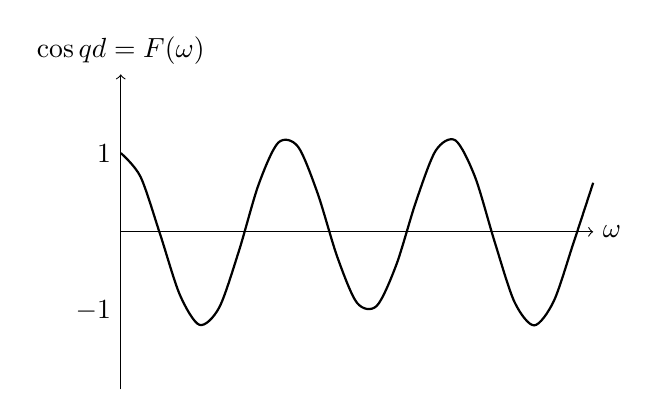
\begin{tikzpicture}
    \draw [->] (0, 0) -- (6, 0) node [right] {$\omega$};
    \draw [->] (0, -2) -- (0, 2) node [above] {$\cos qd=F(\omega)$};

    \draw [thick, domain=0.001:6] plot [smooth] (\x, {cos(deg(\x))*cos(2*deg(\x))-0.5*(2+0.5)*sin(deg(\x))*sin(2*deg(\x))});

    \draw (0,1) node [left] {$1$};
    \draw (0,-1) node [left] {$-1$};
  \end{tikzpicture}
\end{center}
By plotting $\omega$ against $q$, one can obtain a photonic band structure, with the gaps at $q=n\pi/d$. Here, the EM wave is attenuated and does not propagate along $\mathbf{\hat{z}}$. The bandgap occurs since there is no absorption since $\varepsilon_a,\varepsilon_b\in\mathbb{R}$, i.e. the wave is evanescent. 
\end{eg}
\begin{eg}[Photonic nanocavity]
Photonic crystals are easier to fabricate in two dimensions, simply by etching holes into a slab of high $k$ material surrounded by low $k$ material. In such 2D photonic crystals it is also possible to incorporate a defect in which a localised photonic mode can exist that emits within the bandgap of the 2D photonic crystal. This defines a photonic nanocavity.\\[5pt]
One application of such photonic nanocavities is in the field of cavity quantum electrodynamics. It is possible to position a small semiconductor quantum dot (QD), an "artificial atom", within the nanocavity. The emission spectrum is strongly modified if the nanocavity mode is designed to be close to the emission wavelength of the quantum dot (strong-coupling regime).\\[5pt]
The cavity mode can be tuned continuously, for example by adsorption of a self-assembled molecular layer on the surface. The strong interaction between the QD and the cavity mode results in the formation of so-called polariton modes. The lower (upper) polariton branch is cavity (QD)-like for positive detuning and QD(cavity)-like for negative detuning. For zero detuning the strong interaction prevents the crossing of the two dispersion relationships. This allows, for example, to control the exciton lifetime in the nanocavity. 
\end{eg}
\newpage
\subsection{Coherence}
For simplicity, in this discussion the waves will be taken to have scalar
amplitudes. Interference phenomena, diffraction etc, rely on the well defined phase between wavelets (determined by optical path lengths etc.) which are eventually summed for the overall wave amplitude. This can be exact only for purely monochromatic waves - a single, well-defined frequency. However, Fourier Theory means that only infinitely long (in time and space) waves can be purely monochromatic. Real sources and waves (even lasers) are at best `quasi-monochromatic'.
\begin{defi}[Coherence length, width]
Phase registration is lost over a distance $c\tau_c$, where $\tau_c$ is the (temporal) coherence length along the direction of propagation, and over a distance $x_c$, where $x_c$ is the (spatial) coherence width perpendicular to the direction of propagation.
\end{defi}
\begin{defi}[Temporal harmonics and power spectrum]
A time-dependent function $f(t)$ can be described in terms of its temporal harmonics $F(\omega)e^{i\omega t}$.
$$f(t)=\frac{1}{2\pi}\int_{-\infty}^\infty F(\omega)e^{i\omega t}d\omega,\quad F(\omega)=\int_{-\infty}^\infty f(t)e^{-i\omega t}d\omega$$
The power in the frequency range $[\omega,\omega+d\omega]$ is the power spectrum, i.e.
$$P(\omega)d\omega\sim|F(\omega)|^2d\omega$$
\end{defi}
\begin{eg}[Lasers]
For a pure harmonic wave of frequency $\omega_0$, say $f(t)\sim\cos(\omega_0t+\alpha)$:
$$F(\omega)=\frac{1}{2}\int\bigg(e^{i(\omega_0t+\alpha)}+e^{-i(\omega_0t+\alpha)}\bigg)e^{-i\omega t}dt\propto e^{i\alpha}\delta(\omega-\omega_0)+e^{-i\alpha}\delta(\omega+\omega_0)$$
i.e. a pair of delta functions at $\pm\omega_0$.
\end{eg}
\begin{eg}[Spectral lines]\leavevmode
\begin{enumerate}
    \item Lifetime broadening: Unstimulated emission from an isolated, stationary atom can be represented semi-classically as a decaying harmonic wave, beginning at $t = 0$ and characterized by a decay time $\tau_s$ or a scattering frequency $\omega_s = 1/\tau_s$:
    $$F(\omega)=\int_0^\infty e^{i\omega_0t}e^{-\omega_st}e^{-i\omega t}dt=\frac{1}{\omega-\omega_0-i\omega_s}\implies P(\omega)=\frac{1}{(\omega-\omega_0)^2+\omega_s^2}$$
    i.e. $P(\omega)$ is a Lorentzian peak centred on $\omega_0$ and with a linewidth (Full Width Half Maximum) of $2\omega_s$, determined by the decay time $\tau_s$.
    \item Thermal broadening: radiation from atoms moving along the line of sight (w.l.o.g. say $x$-axis) with velocity $v_x$ will be Doppler-shifted in frequency $\omega-\omega_0=\frac{\omega_0v_x}{c}$. The observed frequency spectrum will be a Gaussian since the distribution of atomic/molecular velocities is Gaussian.
    $$P(\omega)=Ce^{-(\omega-\omega_0)^2/2\sigma^2},\quad\sigma^2=\frac{\omega_0^2k_BT}{mc^2}$$
    the full-width half maximum in $\omega$-space will be
    $$2.36\omega_0\sqrt{\frac{k_BT}{mc^2}}=2.36\sigma$$
    \item Pressure broadening: In a gas, an individual atom is subject to collisions with other atoms, which at the very least perturb the phase correlation of the emitted wave before and after each collision. The mean time $\tau_1$ between collisions is:
    $$\tau_1=\frac{1}{4N\overline{v}A}\propto\sqrt{T}/p$$
    where $N$ is the number density of atoms of collision cross-section $A$ and with mean velocity $\overline{v}$, and $p$ is the pressure. This also produces another Lorentzian profile (irrespective of the natural lifetime $\tau$)
    $$P(\omega)\sim\frac{1}{(\omega-\omega_0)^2+1/\tau_1^2}$$
\end{enumerate}
For a gas discharge lamp, the output is the superposition of large numbers of independent photons from individual similar atoms. This is essentially harmonic with frequency $\omega_0$ say, but with an amplitude and phase which have some random fluctuations - quasi-monochromatic light. $\omega_0$ is the underlying harmonic wave, and the linewidth $\Delta\omega$ can be related to some overall broadening equivalent to a lifetime $\tau_s$.
\end{eg}
\begin{eg}[White light]
At the extreme, a large number of atoms of different emission frequencies, or oscillators in the surface of an incandescent black body, result in white light with a very broad power spectrum covering the visible. There is thus zero coherence.
\end{eg}
For a strongly correlated (strongly coherent) waveform, interference effects are very clear. But what about diffraction and interference using a quasi-monochromatic light? It turns out that interference ideas provide a useful quantified description for the degree of correlation, or degree of coherence, of the partially coherent wavefield arising from a light source.
\begin{defi}[Coherence]
Two wave sources are perfectly coherent if their frequency and waveform are identical and their phase difference is constant. This allows us to predict the amplitude and phase of the wavefield at some location $\mathbf{r_2}$ and time $t_2$ from the knowledge of that at location $\mathbf{r_1}$ and time $t_1$.
\end{defi}
\begin{Note}[Optical Stethoscope]
The optical stethoscope is an imaginary device for investigating the time and spatial variation of wavefields and their temporal (on two different wavefronts along the direction of propagation) and spatial coherence (on the same wavefront transverse to the direction of propagation). Two identical optical fibres sample the wavefield at points A$_1$ and A$_2$ and transfer the amplitudes of the wavefield to the closely spaced points B$_1$ and B$_2$ which act as point sources to generate an interference pattern on a screen P. The fibres are lossless and introduce identical phase shifts which can be ignored.
\end{Note}
\begin{defi}[Time average]
The time average for any function $g(t)$ is defined as
$$\langle g(t)\rangle=\lim_{T\rightarrow\infty}\frac{1}{T}\int_0^Tg(t)dt$$
\end{defi}
\begin{defi}[Mutual coherence function]
Suppose we can sample the wavefield $f$ at two different points at different times, i.e. $f_1$ at $\mathbf{r_1}$ at $t$ and $f_2$ at $\mathbf{r_2}$ at $t-\tau$, then the complex mutual coherence function $\Gamma$ is defined as
$$\Gamma(\mathbf{r_1},\mathbf{r_2},\tau)=\langle f_1(\mathbf{r_1},t)f_2^*(\mathbf{r_2},t-\tau)\rangle$$
\end{defi}
\begin{defi}[Degree of mutual coherence]
Normalize the mutual coherence function to yield the degree of mutual coherence
$$\gamma(\mathbf{r_1},\mathbf{r_2},\tau)=\frac{\Gamma(\mathbf{r_1},\mathbf{r_2},\tau)}{\sqrt{I_1I_2}},\quad I_1=\Gamma(\mathbf{r_1},\mathbf{r_1},0),~I_2=\Gamma(\mathbf{r_2},\mathbf{r_2},0)$$
where $I_1$ and $I_2$ are the mean intensities at $\mathbf{r_1}$ and $\mathbf{r_2}$. $\gamma(\mathbf{r_1}, \mathbf{r_2}, \tau)$ determines how effectively the disturbances (wavelets) originating from $\mathbf{r_1}$ and $\mathbf{r_2}$ can interfere. If $I_1$ and $I_2$ are equal and $|\gamma|\sim1$, then $I$ can vary down to zero, giving good fringe contrast, as will become clear.
\end{defi}
\begin{eg}
To investigate 
\begin{itemize}
    \item temporal coherence: compares the wavefield $A_1=f(t)$ at one time with the wavefield $A_2=f(t-\tau)$ at some earlier time, at the `same point' on the wavefront: $\tau\neq 0$, $\mathbf{r_1}=\mathbf{r_2}$. This configuration is an example of amplitude division, i.e. it principally examines the time dependence of the field.
    \item spatial coherence: compares the wavefield $A_1$ at one point $\mathbf{r_1}$ in space with the wavefield $A_2$ at some other point $\mathbf{r_2}$ at the same time and same wavefront: $\tau=0$, $\mathbf{r_1}\neq\mathbf{r_2}$. This configuration is an example of wavefront division, i.e. it principally examines the space dependence of the field.
\end{itemize}
\end{eg}
\newpage
\subsubsection{Temporal coherence}
\begin{defi}[Temporal coherence function]
Define the temporal coherence function for the wavefield to be
$$\Gamma(\tau)=\langle f(t)f^*(t-\tau)\rangle$$
\end{defi}
\begin{Note}
The time delay between the two rays $\tau=2d/c$ can be altered spatially by moving the retro-reflector. The output intensity depends on the spatially introduced time interval $\tau$:
$$I(\tau)=\langle[f(t)+f(t-\tau)][f^*(t)+f^*(t-\tau)]\rangle=2I_0+\langle f(t)f^*(t-\tau)\rangle+\langle f(t-\tau)f^*(t)\rangle=2I_0+2\text{Re}[\Gamma(\tau)]$$
since $\Gamma\in\mathbb{C}$, we have $\Gamma=|\Gamma(\tau)|e^{i\Delta(\tau)}$, then
$$I(\tau)=2I_0+2\text{Re}[\Gamma(\tau)]=2I_0+2|\Gamma(\tau)|\cos(\Delta(\tau))$$
$\Gamma(\tau)$ has an amplitude and a phase term which both depend on the path difference which determines $\tau$.
\end{Note}
\begin{defi}[Fringe visibility]
$$V=\frac{I_{\text{max}}-I_{\text{min}}}{I_{\text{max}}+I_{\text{min}}}$$
\end{defi}
\begin{eg}
If the waveform is quasi-monochromatic, $f(t)\sim e^{-i\omega_0t}=e^{-ik_0ct}$, then
$$\Gamma(\tau)=\langle f(t)f^*(t-\tau)\rangle\sim\frac{1}{T}\int_0^Te^{-i\omega_0t}e^{i\omega_0(t-\tau)}dt\sim e^{-i\omega_0\tau}=e^{-i2k_0d}$$
The phase term oscillates with changes in $d$ on the order of the wavelength of the light - rapidly compared with the variation in the amplitude $|\Gamma(\tau)|$. So if $I(\tau)$ is measured as $\tau=2d/c$ is varied, `fringes' are observed.
\end{eg}
\begin{cor}
$$V(\tau)=|\gamma(\tau)|$$
\end{cor}
\begin{proof}
We have $I_{\text{max}}=2I_0+2|\Gamma(\tau)|$ and $I_{\text{min}}=2I_0-2|\Gamma(\tau)|$, so $V(\tau)=\frac{|\Gamma(\tau|}{I_0}=|\gamma(\tau)|$, where $\gamma(\tau)$ is the normalized temporal coherence function.
\end{proof}
\begin{defi}[Autocorrelation]
The autocorrelation $h(\tau)$ of an irregular normalized waveform $f(t)$ is
$$h(\tau)=\int_{-\infty}^\infty f(t)f^*(t-\tau)dt$$
\end{defi}
\begin{remarks}
$h(\tau)$ is a measure of how $f$ at some time $t$ is correlated with $f$ at some other time. $h(\tau)$ must peak for $\tau=0$.
\end{remarks}
\begin{thm}[Wiener-Khinchine theorem]
$$H(\omega)=|F(\omega)|^2$$
where $H$ and $F$ are Fourier transforms of $h$ and $f$ respectively.
\end{thm}
\begin{proof}
$$H(\omega)=\int\int e^{-i\omega\tau}f(t)f^*(t-\tau)dtd\tau=\int\int e^{-i\omega(\tau+t)}f(t+\tau)e^{i\omega t}f^*(t)dtd\tau=F(\omega)F^*(\omega)$$
\end{proof}
\begin{remarks}
$h(\tau)$ and $\gamma(\tau)$ are similar, and only differ from a normalization factor. The Wiener-Khinchine theorem shows that the fringe visibility $V(\tau)$ for $f(t)$ is directly related to its power spectrum $P(\omega)$. For broadband light sources, no fringes are observable.
\end{remarks}
\begin{cor}
For real $f(t)$, the power spectrum of a light beam can be obtained by Fourier transforming the relative intensity $I_r(\tau)$ observed by introducing a time delay $\tau$ between two beams obtained by amplitude division.
\end{cor}
\begin{proof}
We have 
$$I(\tau)=2I_0+2\text{Re}[\Gamma(\tau)]\implies I_r(\tau)=1+\text{Re}[\gamma(\tau)]$$
since $f(t)\in\mathbb{R}$, we have $\gamma(\tau)=I_r(\tau)-1$. Since the power spectrum $P(\omega)$ is related ot the Fourier transform of $\gamma(\tau)$, it is in turn the Fourier transform of $I_r(\tau)-1$.
\end{proof}
\begin{Note}[Fourier transform spectroscopy]
The optical path of one beam can be varied with respect to the other introducing a measurable time delay $\tau=2d/c$. The compensator plate, identical to that forming the beamsplitter, ensures that the both optical paths are equivalent when the movable mirror is the same distance $d_0$ from the beamsplitter as is the fixed mirror. One beam is reflected internally at the beamsplitter, and one externally, which introduces a phase difference of $\pi$ which can be ignored.
\end{Note}
\begin{defi}[Coherence length and time]
We define the coherence length $\ell-c$ as the path difference $(2d)$ at which the visibility falls by a factor of $e$. $\ell_c$ is a measure of coherence time $\tau_c=\ell_c/c$.
\end{defi}
\begin{eg}[Broadened spectral line]
Suppose the power spectrum $P(\omega)$ has a Gaussian profile $P(\omega)\propto e^{-(\omega-\omega_0)^2/2\sigma^2}$. We obtain $\Gamma(\tau)$ from the Wiener-Khinchine theorem:
$$\Gamma(\tau)\sim \int e^{i\omega\tau}e^{-(\omega-\omega_0)^2/2\sigma^2}d\omega=e^{i\omega_0\tau}\int e^{iu\tau}e^{-u^2/2\sigma^2}du\sim e^{i\omega_0\tau}e^{-\sigma^2\tau^2/2}$$
where $u=\omega-\omega_0$. But $I(\tau)=2I_0+2|\Gamma(\tau)|\cos(\omega_0\tau)$, so
$$I_r=1+\exp(-\sigma^2\tau^2/2)\cos(\omega_0\tau)$$
so the visibility is $V(\tau)=e^{-\sigma^2\tau^2/2}$. The interferogram shows essentially the same fringes as for a truly monochromatic source, but the fringe visibility falls as $d$ increases. The spacing of the fringes ($I \sim\cos(2d\omega_0/c)$) gives the central frequency $\omega_0$ of the line. The visibility gradually decreases as the $d$ increases because the two beams are becoming less mutually coherent. The coherence length (directly measurable from the interferogram) is $\ell_c\approx c\sqrt{2}/\sigma$, where $\sigma$ determines the frequency linewidth $\delta\omega$ of the spectral line. $\delta\omega$ is usually the full width half maximum of the Gaussian profile $P(\omega)$.
$$2.36\sigma=\delta\omega\sim c\delta k=2\pi c\delta(1/\lambda)\sim 2\pi c\frac{\delta\lambda}{\lambda^2}$$
And hence the coherence length is
$$\ell_c\approx\frac{c\sqrt{2}}{\sigma}\sim\frac{2.36}{\pi\sqrt{2}}\frac{\lambda^2}{\delta\lambda}$$
For Kr$^{84}$ line, $\lambda=560$ nm with $\delta\lambda\sim 0.0002$ nm and so $\ell_c\sim 0.78$ m.
\end{eg}
\begin{remarks}
Fourier transform spectroscopy is particularly powerful in the infrared spectral range. FTIR (Fourier transform infrared spectroscopy) has two important advantages over conventional infrared spectrometers that use monochromators / diffraction gratings:
\begin{itemize}
    \item The radiation throughput is higher because it is not limited by the input slit width; the size of the detector in an FTIR can be as large as the central interference ring (Jacquinot advantage).
\item The signal-to-noise ratio is higher because as the mirror separation is scanned the signal is continuously falling on the detector. In contrast, in a grating spectrometer, only background signal is falling on the detector while the monochromator switches between wavelengths (Fellgett advantage).
\end{itemize}
The spectral resolution of a Fourier transform spectrometer is given by $\frac{\lambda}{\delta\lambda}=2\times m$, where $m$ is the number of fringes recorded (limited by the size of the spectrometer).
\end{remarks}
\begin{Note}[Spatial observation of temporal coherence]
A broadened spectral line source with coherence length $\ell_c=c\tau_c$ affects the fringes obtained with Young's slits. Waves at P from slits illuminated with a parallel beam have path lengths which differ by $\ell$. They become decreasingly mutually coherent as $\ell\rightarrow\ell-c$ and beyond, so the fringe visibility will decrease as P moves off-axis.
\end{Note}
\newpage
\subsubsection{Spatial coherence}
\begin{Note}[Extended source for double slit]
Young's slits illuminated not by a parallel beam but a beam of
wavelength $\lambda$ and finite angular width from an extended source with intensity variation $I(x)$ in its own plane. Each point on the source produces a set of $\cos^2$ fringes angularly offset from each other because of the different angles the points on the source make at O. So the fringe contrast on the screen is degraded. If the angular width of the source measured from O is $\alpha$, then the fringes from the two edges will be offset by $\alpha D$. The spacing of each set of fringes is $\lambda D/d$, so serious contrast degradation sets in if:
$$d>\frac{\lambda}{\alpha}\approx w_c$$
where $w_c$ is the coherence width. For the two rays shown:
$$r_{1,2}+\rho_{1,2}=\rho+R\pm\frac{d}{2}\sin\theta\pm\frac{d}[2]\sin\chi$$
Now take $\sin\theta\approx x/L$ and $\sin\chi\approx y/D$, so the phase difference for the rays arriving at P from the point $x$ is 
$$k(r_1+\rho_1-r_2-\rho_2)=kd(\sin\theta+\sin\chi)=kd\bigg(\frac{x}{L}+\frac{y}{D}\bigg)=2ks$$
The amplitude $\psi(y)$ at P arising from the source region $x\rightarrow x+dx$ is then
$$\psi(y)\sim e^{ik(\rho+R)}\sqrt{I(x)}(e^{iks}+e^{-iks})=e^{ik(\rho+R)}\sqrt{I(x)}2\cos kx$$
where $I(x)$ is the intensity profile of the source. If the extended source is incoherent (radiation from each point on it is uncorrelated with that from any other point), the net intensity at P is obtained by summing $\sum|\psi(y)|^2$:
$$I_y(d)=\int|\psi(y)|^2dx=2\int I(x)(1+\cos2 ks)dx=2I_0+2\text{Re}\bigg[e^{-ikdy/D}\int I(x)e^{-ikdx/L}dx\bigg]$$
Change variables $x\approx L\theta$, $y\approx D\chi$, so $I(x)dx\rightarrow I(\theta)d\theta$ and write $kd=u$, then the intensity on the screen as a function of $y$ and of the slit separation $d$ is
$$I_y(u)=2I_0+2I_0\text{Re}[e^{iu\chi}\gamma(u)],\quad\gamma)u)=\frac{1}{I_0}\int I(\theta)e^{-iu\theta}d\theta$$
Write $\gamma(u)=|\gamma(u)|e^{-i\beta}$, then since $u\chi=kyd/D$, then
$$\gamma_y(u)=2I_0+2I_0|\gamma(u)|\cos\bigg(\beta+\frac{kyd}{D}\bigg)$$
The offset $\beta$ is determined by the source angular profile $I(\theta)$.
\end{Note}
\begin{figure}[H]
    \centering
    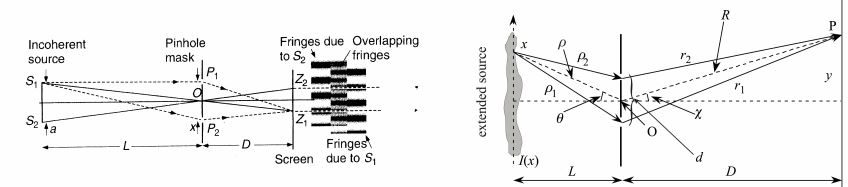
\includegraphics[width=\linewidth]{spatialcoherence.JPG}
\end{figure}
This motivates the following theorem:
\begin{thm}[van Cittert-Zernike theorem]
The degree of lateral coherence is the Fourier transform of the angular intensity distribution of the source $I(\theta)$.
$$\gamma(u)=\frac{1}{I_0}\int I(\theta)e^{-iu\theta} d\theta=\frac{\mathcal{F}[I(\theta)]}{I_0}$$
\end{thm}
\begin{eg}
When $I(x)$ is symmetric about the axis of the system, $\gamma(u)\in\mathbb{R}$ and $\beta=0$ if $\gamma(u)>0$, $\beta=\pi$ if $\gamma(u)<0$. The visibility of the fringes is then $V=\gamma(u)$ when $u=kd$.
\end{eg}
\begin{eg}
Suppose the slits are illuminated by a distant, uniform line source (parallel to the slits) of angular width $\alpha$, i.e. $I(\theta)=J$ if $-\alpha/2\leq\theta\leq\alpha/2$, then
$$\gamma(u)=\frac{1}{I_0}\int_{-\alpha/2}^{\alpha/2}Je^{-iu\theta} d\theta=\sinc\frac{u\alpha}{2}$$
where $I_0=\alpha J$. The observed fringe contrast depends on $u\alpha/2$ and falls to zero at $u\alpha/2=\pi\alpha d/\lambda=\pi$ at $d=\lambda/\alpha$, beyond which $V$ becomes negative.
\end{eg}
\begin{eg}
A disc source of angular diameter $\alpha$ illuminating two pinholes separated by $d$, gives
$$\gamma(u)=\frac{2J_1(u\alpha/2)}{u\alpha/2}$$
For this circular symmetry, the fringe visibility falls to zero for $u\alpha/2=3.83$, and the coherence width is then $w_c=1.22\lambda/\alpha$.
\end{eg}
\begin{remarks}
The broader the source, the narrower the coherence width.
\end{remarks}
\begin{Note}
How does the fringes obtained for two pinhole apertures (hence the envelope profile) depend on their separation $d$ for fixed source width. As $d$ is increased, the fringe spacing falls, as does the fringe contrast, as the two pinholes becomes less mutually coherent. Due to the `sinc' form of the $\gamma(u)$ function, $V$ in fact goes through zero and then rises slightly.
\end{Note}
\begin{remarks}
In 2D, one can define a coherence area. Further account for temporal coherence gives us the coherence volume.
\end{remarks}
\begin{eg}
For sunlight ($\lambda\sim 500$ nm, $\delta\lambda\sim 500$ nm, $\alpha\sim 0.5\degree$), we have the coherence width and coherence length to be
$$w_c\sim\frac{\lambda}{\alpha}\sim 5\times10^{-5}m,\quad\ell_c\sim\frac{\lambda^2}{\delta\lambda}\sim 500 nm$$
For distant stars, $\alpha<<0.01$ radians, so their coherence widths at the Earth are much greater and can be exploited to measure their angular diameters.
\end{eg}
\begin{Note}[Michelson's stellar interferometer]
Since $\alpha$ is very small for stars, $w_c$ is several metres for visible wavelengths. Using a Young's slit set-up to observe the reduction in fringe contrast as $d$ is increased is impossible, as fringes with very small spacing would result. We may achieve variable large spacing $D$ using moveable mirrors to focus light to the fixed slits. The fringe visibility as a function of $D$ allows coherence widths on the scale of metres to be measured.
\end{Note}
\begin{eg}
Michelson used this to look at the star Betelgeuse. For $\lambda = 570$ nm, the fringes vanished at $D = 3.07$ m, corresponding then to $\alpha=22.6\times10^{-8}$ rad (0.047 sec of arc). Using the distance from the Earth determined independently by parallax measurements, this can be used to determine the diameter of the star, which is 950-1200 times the radius of the Sun.\\[5pt]
To create an image of the star one needs to know not the magnitude of the coherence function $|\gamma|$ but also its phase $\beta$. The difficulty in determining $\beta$ is that it is affected also by atmospheric jitter that can cause shifts of the interference pattern with respect to the optical axis of the telescope. To overcome this more than two entrance apertures, at least three apertures A$_1$, A$_2$ and A$_3$ can be used. If the apertures are selected such that the pairs A$_1$A$_2$, A$_2$A$_3$ and A$_1$A$_3$ produce interference fringes with different periods that can be measured simultaneously, the atmospheric phase shifts can be eliminated and the real phase of $\gamma$ can be determined (method of phase closure). This allows reconstructing an image of the star through Fourier transformation.
\end{eg}
\newpage
\section{Electrodynamics}
\subsection{Vector Potential from classical EM}


\newpage
\subsection{Vector Potential for quantum mechanics}

\newpage
\subsection{General solution for potentials}
\newpage
\section{Dipole Radiation}
\subsection{Hertzian dipole}

\newpage
\subsection{Multipole expansion in the far field}
\newpage
\section{Antenna}

\newpage
\section{Light Scattering}
\subsection{Polarization of Scattered Waves}
\subsection{Various Scattering Mechanisms}
%Rayleigh, Thomson, Raman

\newpage
\section{Relativistic Electrodynamics}

\newpage
\section{Radiation}
\end{document}